This chapter contains a summary of the concepts, definitions and results this thesis is based on. These include the definition and relevance of image moments (for both grayscale and color images), with special emphasis on Zernike moments. Moment invariants with respect to image rotation, translation and scaling are introduced.
Moreover, the algebra of quaternions is also introduced and is used as a tool to generalize grayscale image moments to color images.
Finally some examples of the state-of-the-art applications in image analysis are presented.

\section{Image moments for grayscale images}\label{sec:grayscale}
In general, image moments are certain descriptive values calculated using the pixel intensities of an image. 

Traditionally, these image moments are defined for grayscale images, where pixel values are described by a single (gray) channel. A grayscale image can be thought of as a discrete sampling of a real valued, two-dimensional function $f : \R^2 \rightarrow \R$, where the function values at a point $(x,y) \in \R^2$ describe the pixel intensity at that point~\cite{moment_book}.

Using this approach, the regular (geometric) image moments $M_{ij}$ can be defined as
\begin{gather} \label{eq:regular_moment}
M_{ij} = \sum_x \sum_y x^iy^jf(x,y),
\end{gather} where $(x,y)$ are the discrete pixel coordinates.
These geometric moments can be used to calculate the centroid of a grayscale image as 
\begin{gather} \label{eq:centroid}
\left\{ \overline{x}, \overline{y} \right\} = \left\{ \frac{M_{10}}{M_{00}},  \frac{M_{01}}{M_{00}} \right\}.
\end{gather}

In more general terms, image moments with order $p$ and repetition $q$ can be defined using a set of basis functions $\left\{H_{pq}\right\}$. Now considering $f$ as a continuous function, moments are defined as
\begin{equation}\label{GeneralMoments}
\iint\limits_A H_{pq}(x,y)f(x,y)\ dx\ dy,
\end{equation} where $A$ is the region of the plane, which contains the image (the domain of $f$).

By choosing the set of basis functions appropriately, many different kinds of image moments can be defined. Each of these moments has applications that utilize certain special properties of the basis functions. For example, some of these moments are Fourier-Mellin moments~\cite{qfmm}, Chebyshev-Fourier moments~\cite{chebyshev-fourier}, radial harmonic Fourier moments~\cite{fourier}, and Zernike moments~\cite{zernike_moments}. The latter of these is defined in detail later in this section.

\subsection{Invariance properties}
Certain image moments, or some combination of moments of different orders can be invariant with respect to image transformations, such as rotation, scaling, and translation (RST transformations).

\paragraph{Rotation invariance.} To define what is meant by rotation invariance, it is useful to consider the image function $f$ defined in polar coordinates. Then the image $f_{r}$, rotated by some degree $\alpha$ can be written as $f_{r}(r,\theta) = f(r,\theta - \alpha)$. A moment invariant achieves rotation invariance, when the moments of $f$ and $f_{r}$ are the same for all possible values of $\alpha$.   

\paragraph{Scaling invariance.} The scaled image $f_{s}$ can be defined as $f_{s}(r, \theta) = f(r / \lambda, \theta)$ for some scaling factor $\lambda > 0$. A moment invariant is said to achieve scaling invariance, when the moments for $f$ and $f_{s}$ are identical. In practice, this means that scaling the image, such that the scaled image is still within the region of the plane over which the moments are defined, does not change the values of the moment invariants.

\paragraph{Translation invariance.} To define translation invariance, it is useful to consider the image in Cartesian coordinates. The image translated by $(x_0, y_0)$ is defined as $f_{t}(x,y) = f(x - x_0, y - y_0)$. Again, similarly to the other types of invariance, a moment invariant is said to be translation invariant if its values for $f$ and $f_{t}$ are the same. Practically, this means that however the image is translated on the plane, as long as it is within the region of the plane over which the moments are defined, the moment invariant values do not change.

\paragraph{RST invariance.} A moment invariant is called RST invariant if it satisfies the criteria for all three previously described kinds of invariance at the same time. 


Translation invariance is generally the easiest to achieve, as translating the image such that the centroid falls on the origin neutralizes any prior translation. The other two kinds of invariance require some special properties of the basis function set or some special construction and combination of the moments.


The exact construction of RST invariant moments for Zernike moments is presented in detail in Section~\ref{sec:qzm}


These invariance properties are widely utilized in applications for pattern matching and image recognition~\cite{app1, app2, app3}. In particular, moment invariants can be used in medical applications, such as solving the Pathological Brain Detection problem~\cite{med_app_1}.


\subsection{Zernike moments}
As mentioned previously, Zernike moments are image moments, defined by choosing the set of basis functions as the Zernike functions. This set of functions (defined later in this section) proved to be a suitable basis for series expansion in numerous optical applications (see for example~\cite{wavefront,optical_human_eye,opt_surf}), and moment invariants could easily be constructed, especially for rotation invariance.


Zernike functions, first introduced by F. Zernike~\cite{zernike} in 1934, are a set of complex functions defined on the unit disk. Since the domain of these functions is the unit disk, it is useful to define them in terms of polar coordinates. The Zernike functions $V_{n,m}$ ($n \in \mathds{N}$, $m \in \mathds{Z}$, $n \geq |m|$ and $n - |m|$ is even) are defined as
\begin{equation}\label{ZernikeFunction}
  V_{n,m}(r,\theta) = R_{n,m}(r) e^{i m\theta} \ \ \ (r\in[0,1], \theta\in[0,2\pi]),
\end{equation}
where $R_{n,m}$ is the radial part and $e^{i m\theta}$ is the azimuthal part of the function. The radial part is defined as the following radial polynomials (of degree $n$)
\begin{gather}
    R_{n,m}(r) = \sum_{k=0}^{\frac{n - |m|}{2}}\frac{(-1)^k (n - k)!}{k!\left(\frac{n + |m|}{2} - k\right)!\left(\frac{n - |m|}{2} - k\right)!}r^{n-2k} \label{eq:radial_poly}.
\end{gather} 


The set of Zernike functions is orthogonal over the unit disk with respect to the weight $r$~\cite{zernike_moments}, so for indices where $n - |m|$ and $n' - |m'|$ are both even we get
\begin{equation}\label{Zortho}
	\int_0^{2\pi}\int_0^1 V_{n,m}(r,\theta)V_{n',m'}^*(r,\theta)r\ dr d\theta  = \frac{\pi}{n + 1}\delta_{n,n'}\delta_{m,m'},
\end{equation}
where $\delta_{a,b}$ denotes the Kronecker delta function, and $V_{n,m}^{*}(r,\theta)$ is the complex conjugate of the Zernike functions, meaning
\begin{gather*}
    V_{n,m}^{*}(r,\theta) = R_{n,m}(r) e^{-i m\theta}.
\end{gather*}

It is important to note that the radial polynomials $R_{n,m}$ are the same for both $m$ and $-m$, so $R_{n,m}(r) = R_{n,-m}(r)$. These radial polynomials also satisfy an orthogonality relation over $[0,1]$ with respect to the weight $r$~\cite{schipp}, that is, for a fixed $m$ we have
\begin{equation}\label{Rortho}
	\int_0^1 R_{n,|m|}(r) R_{n',|m|}(r)r\ dr  = \frac{1}{2n+2} \delta_{n,n'}.
\end{equation}


Another important and useful property of these radial polynomials is that they can be expressed in terms of the shifted Jacobi polynomials. Let $P_k^{(\alpha, \beta)}(x)$ denote the $k$-th degree classical Jacobi polynomials~\cite{Szego}. The Jacobi polynomials are the set of polynomials defined over $[-1,1]$, which are orthogonal with respect to the weight $(1-x)^\alpha(1+x)^\beta$. By shifting the argument of these polynomials, we can get polynomials which are defined over $[0,1]$, the domain of the radial polynomials $R_{n,m}$. Expressing these radial polynomials in terms of the shifted Jacobi polynomials we get
\begin{equation}\label{RJacobi}
	R_{n,m}(r) = r^{|m|} P_{\frac{n - |m|}{2}}^{(0,|m|)}(2r^2-1).
\end{equation} 


Let $f(r,\theta)$ be a grayscale, continuous image function (given in polar coordinates), whose domain is the unit circle.
Using the previously defined set of Zernike functions, the Zernike moment of order $n$, repetition $m$ of $f(r,\theta)$ can be defined as
\begin{gather}\label{eq:complex_zernike_def}
    Z_{n,m}(f) = \frac{n + 1}{\pi}\int_0^1\int_0^{2\pi}f(r,\theta)V_{n,m}^{*}(r,\theta)r\ dr\ d\theta.
\end{gather}


By utilizing the orthogonality of the Zernike functions, the original image function $f(r,\theta)$ can be approximately reconstructed from a finite number of Zernike moments up to degree $M$:
\begin{gather}\label{eq:reconstruction}
    f(r,\theta) \approx \sum_{n=0}^{M}\sum_{m=-n}^{n}Z_{n,m}(f)V_{n,m}(r,\theta).
\end{gather}

\paragraph{Invariance properties of Zernike moments.} Translation invariance (as described previously) can be achieved by translating the image such that the centroid of the image falls on the origin. This method is suitable to use with Zernike moments as well.


To calculate rotation invariant features from Zernike moments, first consider the moments of an image rotated by some degree $\alpha$, defined using polar coordinates: $f_{r}(r,\theta) = f(r,\theta - \alpha)$. In this case it can be shown that
\begin{gather*}
    Z_{n,m}(f_r) =  Z_{n,m}(f) e^{-i m\alpha}.
\end{gather*}
This means that the modulus Zernike moments is the same regardless of how the image is rotated, thus $|Z_{n,m}(f)|$ are rotation invariant features~\cite{zernike_moments}.


Scaling invariance is discussed in detail in Section~\ref{sec:qzm}, for quaternion Zernike moments.

\section{Image moments for multichannel, color images}
The image moments in Section~\ref{sec:grayscale} are only defined for single-channel, grayscale images. Extending these signal and image processing techniques efficiently to multichannel color images is an important and generally unresolved problem. This section introduces some conventional approaches to generalize the grayscale methods to RGB images. Later, the algebra of quaternions is also presented, and using this algebra, quaternion moments are introduced, specifically quaternion Zernike moments and their invariant properties.  

\subsection{Conventional techniques}
The two main approaches used both rely on using the grayscale method in some form. One method is to use grayscale conversion to convert the RGB image to a single-channel grayscale image and use the grayscale method on this converted image. The drawback of this method is that the color information contained in multiple channels is lost. Thus, for example, this method cannot distinguish between a red and a blue object.

The other main conventional method utilizes RGB-decomposition, whereby the grayscale (single-channel) method can be used on each of the individual color channels~\cite{affine_color}. This approach does not lose color information, but any relationship between the color channels cannot be utilized by the method.


\subsection{Algebra of quaternions}
More recently, the algebra of quaternions was employed to generalize various single-channel moments, so that color images can be analysed holistically. In order to introduce this generalization, we first introduce the algebra of quaternions and how color images can be represented as quaternion valued functions.


Quaternions were defined by Hamilton~\cite{Hamilton} as a generalization of the complex numbers. The set of quaternions is denoted by $\Hq$. A quaternion, $q \in \Hq$, consists of four components:
\[
	q = a+b\qi +c\qj+d\qk,
\]
where $a,b,c$ and $d$ are real numbers, and $\qi,\qj,\qk$ are the imaginary units, defined according to the following rules:
\[
\begin{gathered}
	\qi^2 = \qj^2 = \qk^2 = \qi\qj\qk = -1,\\
	\qi\qj = -\qj\qi = \qk,\ \qj\qk = -\qk\qj = \qi,\ \qk\qi = -\qi\qk = \qj.
\end{gathered}
\]
Therefore, the set of quaternions $\Hq$ is an \textit{algebra}. It is important to note, that the multiplication of quaternions is not commutative. The conjugate and modulus of $q$ are respectively defined by
\[
\begin{gathered}
q^* = a-b\qi-c\qj-d\qk, \\
|q| = \sqrt{a^2+b^2+c^2+d^2}.
\end{gathered}
\]

A quaternion is called pure quaternion, when $a = 0$, i.e. the real part of the quaternion is zero. $q$ is called a unit quaternion if $|q| = 1$.

\paragraph{Representing color images with quaternions.}
The 3-dimensional RGB color space can be thought of in terms of pure quaternions, where the color $(r,g,b)$, consisting of the three components $r,g,b \in [0,1]$, is uniquely described by the pure quaternion $r\qi + g\qj + b\qk$.


In practice, quaternions are useful for describing three-dimensional rotations, thus rotations in the RGB color space can be easily described by representing the colors in terms of pure quaternions.


\citeauthor{EllSangwine} \cite{EllSangwine} utilized quaternions to represent a color image, $f: \R^2\to\R^3$ , as follows:
\[
f(x,y) = \qi f_R(x,y) + \qj f_G(x,y) + \qk f_B(x,y),
\]
where functions $f_R , f_G, f_B:\R^2\to\R$ represent the red, green and blue components of the $(x,y)$ pixel, respectively. This way, a color image can be thought of as a pure quaternion valued function and the algebra of quaternions can be employed to define image moments in a similar manner as in the case of grayscale images.

\subsection{Quaternion moments}
Similar to the general formula for defining the moments of grayscale images in \eqref{GeneralMoments}, quaternion moments can be defined by a set of quaternion valued basis functions and a quaternion valued, continuous image function. Most commonly, the set of complex valued basis functions is generalized such that we get a set of quaternion valued basis functions.

For example, \citeauthor{qfmm}~\cite{qfmm} introduced quaternion Fourier-Mellin moments (QFMMs) which are an extension of the conventional Fourier-Mellin moments. Similarly, the same quaternion techniques were applied successfully to other function systems (e.g.~\cite{Shao, chebyshev-fourier}), yielding similar results.

\subsection{Quaternion Zernike moments}\label{sec:qzm}
\citeauthor{qzm}~\cite{qzm,qzmi} proposed the quaternion Zernike moments (QZMs), an extension of the conventional Zernike moments to color images using quaternions. Generally, this method overperforms other similar approaches in color image recognition, due to the natural invariances of Zernike functions.


Quaternion Zernike moments, just like regular Zernike moments, are defined over the complex unit disk
\[
	\D = \left\{ z = re^{i\theta}\in\C \ :\ r\in[0,1],\theta\in[0,2\pi)\right\}.
\]


In order to define quaternion Zernike moments, first we have to define the quaternion-valued generalization of the complex-valued Zernike functions defined in \eqref{ZernikeFunction}. Since the radial part of the Zernike functions is a real-valued function of $r$, only the azimuthal component needs to be generalized. Thus the quaternion-valued Zernike functions can be defined as
\[
	\phi_{n,m}(r,\theta) = R_{n,m}(r) e^{-\qmu m\theta},
\]
where $\qmu$ is an arbitrary unit pure quaternion. The usual choice for $\qmu$ is the value $\frac{\mathbf{i} + \mathbf{j} + \mathbf{k}}{\sqrt{3}}$, because this is the unit pure quaternion representing the color gray in the RGB color space.

Similarly to the complex-valued Zernike functions, the generalized Zernike functions also satisfy the following orthogonality relation with respect to the weight $r$:
\begin{equation}\label{QZortho}
	\frac{n+1}{\pi} \int_0^1 \int_0^{2\pi} \phi_{n,m}(r,\theta) \phi^*_{n',m'}(r,\theta) r \ d\theta dr = \delta_{n,n'}\delta_{m,m'}.
\end{equation}


Let $f(r,\theta)$ be a pure quaternion valued RGB image function with a continuous domain, defined in polar coordinates over the unit disk $\D$. As described previously, each color component of the image function corresponds to one of the imaginary units.


The definition of QZMs is similar to the definition of Zernike moments in \eqref{eq:complex_zernike_def}, but instead of the complex-valued $V_{n,m}$ functions we use the generalized $\phi_{n,m}$ functions. Since the multiplication of quaternion is not commutative, both right-side and left-side quaternion Zernike moments can be defined, depending on which side we multiply $f(r,\theta)$ from. The right-side QZM of order $n$ and repetition $m$ is defined as
\begin{gather}
    \begin{split}
    Z_{n,m}^R(f) &= \frac{n + 1}{\pi}\int_0^1\int_0^{2\pi}R_{n,m}(r)f(r,\theta)e^{-\bm{\mu}m\theta}r\ dr\ d\theta, \\
    &n \geq |m| \text{  and  } n - |m| \text{  is even,}
    \end{split}
    \label{eq:QZRM}
\end{gather}
while the left-side QZM for the same indices is defined as 
\begin{gather*}
Z_{n,m}^L(f) = \frac{n + 1}{\pi}\int_0^1\int_0^{2\pi}R_{n,m}(r)e^{-\bm{\mu}m\theta}f(r,\theta)r\ dr\ d\theta.
\end{gather*}


Analogously to the grayscale case in \eqref{eq:reconstruction}, the image function $f(r,\theta)$ can be approximated by using either right-side or left-side QZMs up to a finite $M$ degree. 
\begin{gather}
    \begin{split}
      f(r,\theta) &\approx \sum_{n=0}^{M}\sum_{m=-n}^{n}Z_{n,m}^R(f)R_{n,m}(r)e^{\bm{\mu}m\theta} \\
      f(r,\theta) &\approx \sum_{n=0}^{M}\sum_{m=-n}^{n}e^{\bm{\mu}m\theta}Z_{n,m}^L(f)R_{n,m}(r)
    \end{split}\label{eq:qzm_reconstruction}
\end{gather}


It is important to note that a left-side QZM can be expressed in terms of the right-side QZM of the same order and repetition using the following relation:
\begin{gather*}
    Z_{n,m}^L(f) = -(Z_{n,m}^R(f))^{*}
\end{gather*}
Because of this, in this thesis only the right-side QZMs will be studied.

\subsubsection{Quaternion Zernike moment invariants}\label{sec:invariance}
\citeauthor{qzmi}~\cite{qzm, qzmi} proposed the constructions described in this section in order to create rotation, scaling and translation invariant moment invariants using the quaternion Zernike moments.

\paragraph{Rotation invariance.}
In order to achieve rotation invariance consider the image rotated by some degree $\alpha$: $f_{r}(r,\theta) = f(r, \theta - \alpha)$. \citeauthor{qzmi}~\cite{qzmi} proved that for the rotated image $Z_{n,m}^R(f_{r}) = Z_{n,m}^R(f)e^{-\bm{\mu}m\theta}$ and $Z_{n,m}^L(f_{r}) = e^{-\bm{\mu}m\theta}Z_{n,m}^L(f)$. 


Similarly to the complex-valued case, the modulus $|Z_{n,m}^R(f)|$ can be used to achieve rotation invariance~\cite{qzm}, but this provides only one real-valued invariant, whereas the following construction can provide quaternion-valued invariants. 


Based on the properties of the QZMs of a rotated image, it follows that the quaternion defined as
$$\Phi_{n,k}^m(f) = Z_{n,m}^R(f)Z_{k,-m}^L(f) = -Z_{n,m}^R(f)(Z_{k,m}^R(f))^*$$
is invariant under rotation, meaning that $\Phi_{n,k}^m(f) = \Phi_{n,k}^m(f_{r})$.
From now on in this thesis, this invariant will be referred to as a quaternion Zernike moment rotation invariant (QZMRI).

\paragraph{Translation invariance.}
Analogously to the construction of translation invariant Zernike moments in the grayscale case, now translation invariance can be achieved by setting the origin of the coordinate system as the centroid of the image.


For grayscale images the centroid can be defined as in \eqref{eq:centroid}. For RGB images, we need the common centroid of all three color channels. This can be calculated using zero-order and first-order geometric moments for each individual color channel, as described by \citeauthor{affine_color}~\cite{affine_color}:

\begin{gather} \label{eq:common_centroid}
    \left\{\overline{x}, \overline{y}\right\} = \left\{\frac{M_{10}^R + M_{10}^G + M_{10}^B}{M_{00}^R + M_{00}^G + M_{00}^B}, \frac{M_{01}^R + M_{01}^G + M_{01}^B}{M_{00}^R + M_{00}^G + M_{00}^B} \right\},
\end{gather}
where $M_{ij}^R, M_{ij}^G, M_{ij}^B$ denote the $M_{ij}$ geometric moments (defined in \eqref{eq:regular_moment}) for the red, green, and blue color channels respectively.


Consider a translated image function in Cartesian coordinates: $f_t(x,y) = f(x - x_0, y - y_0)$. 

If the origin of the coordinate system is placed on the common centroid of the color channels $(\overline{x}, \overline{y})$, then the QZMs calculated in this coordinate system will be invariant to translation. This further translated image is denoted by $\overline{f_t}(x,y) = f_t(x - \overline{x}, y - \overline{y})$. Note that the common centroid of $f_t$ and $f$ are different, thus these two images need to be further translated by different amounts.


By considering the QZMs of both $\overline{f_t}$ and $\overline{f}$, we get
\begin{gather*}
    {Z}_{n,m}^R\left(\overline{f_t}\right) = {Z}_{n,m}^R\left(\overline{f}\right).
\end{gather*}


This means that first translating the image so that the common centroid falls on the origin of the coordinate system and only then calculating the QZMs yields translation invariance. 
Let $\overline{Z}_{n,m}^R\big(f\big) = {Z}_{n,m}^R\left(\overline{f}\right)$ denote these translation invariant QZMs.

\paragraph{Scaling invariance.}
For non-negative integers $m$ and $l$, \citeauthor{qzmi}~\cite{qzmi} constructed scaling invariants utilizing the symmetric property of the radial polynomials with respect to $m$ and an alternate form of the QZMs.


Let $f_s(r,\theta) = f(r/\lambda, \theta)$ denote an image scaled with some $\lambda > 0$ scaling parameter. It was shown that the QZMs of the scaled image can be expressed as a linear combination of the QZMs of the original image in the following way:

\begin{gather*}
  \begin{split}
  c_{m,l}^{t,k} &= (-1)^{l-k}\frac{(m + 2l + 1)(m + k + l)!}{(l - k)!(k - t)!(m + k + t + 1)!} \\
  Z_{m + 2l,m}^R(f_s) &= \sum_{t=0}^l\sum_{k=t}^l\lambda^{m+2k+2}c_{m,l}^{t,k}Z_{m+2t,m}^R(f).
  \end{split}
\end{gather*}

Utilizing the formula above, the following scaling invariants have been constructed:


\begin{gather*}
    L_{m + 2l,m}^R(f) = \sum_{t=0}^l\sum_{k=t}^l\left(\sqrt{|Z_{0,0}^R(f)|}\right)^{-(m+2k+2)}c_{m,l}^{t,k}Z_{m+2t,m}^R(f).
\end{gather*}

These scaling invariants satisfy $L_{m + 2l,m}^R(f_s) = L_{m + 2l,m}^R(f)$, meaning that their values are the same regardless of how the original image was scaled.


\paragraph{Combined RST invariants.}
Similarly to the construction of the rotation invariants $\Phi_{n,k}^m$, the previously defined scaling invariants can also be used to construct $\Psi_{n,k}^m(f) = L_{n,m}^R(f)(L_{k,m}^R(f))^*$, which is invariant to both rotation and scaling.


In order to achieve translation invariance as well, throughout the construction of the scaling invariants $L_{n,m}^R$ the translation invariant QZMs ($\overline{Z}_{n,m}^R(f)$) can be used, thus defining the $\overline{L}_{n,m}^R$ combined translation and scaling invariants. This means that before constructing the scaling invariants, the image has to be translated so that the combined centroid falls on the origin.


Finally, to achieve combined RST invariance, the combined translation and scaling invariants can be used to construct $\overline{\Psi}_{n,k}^m(f) = \overline{L}_{n,m}^R(f)(\overline{L}_{k,m}^R(f))^*$, which is invariant to rotation, scaling, and translation. These $\overline{\Psi}_{n,k}^m(f)$ values are called quaternion Zernike moment invariants (QZMI).


\subsection{Quaternion radial harmonic Fourier moments}
Another set of quaternion-valued moments are the quaternion radial harmonic Fourier moments (QRHFMs)~\cite{Wang, WangAcc, LiuAcc}. We introduce and describe these moments, as in Chapter~\ref{sec:tests} we present comparisons between the capabilities of QRHFMs and QZMIs.


Similarly to Zernike moments, these Fourier moments are also defined for images whose domain is the unit disk $\D$. The basis functions for QRHFMs are defined as
\begin{gather*}
    H_{n,m}(r,\theta) = R_n(r)e^{\qmu m \theta},
\end{gather*}
where $\qmu$ is a unit pure quaternion, usually $\qmu = \frac{\mathbf{i} + \mathbf{j} + \mathbf{k}}{\sqrt{3}}$, and $R_n(r)$ are the radial kernel functions defined as
\begin{gather*}
    R_n(r) = \begin{cases}
        \frac{1}{\sqrt{r}}, &n = 0\\
        \sqrt{\frac{2}{r}}\cos(\pi n r), &n \text{ is even}\\
        \sqrt{\frac{2}{r}}\sin(\pi (n+1) r), \ \ &n \text{ is odd}
    \end{cases}.
\end{gather*}

The functions $H_{n,m}(r,\theta)$ also satisfy the following orthogonality relation:
\begin{gather*}
     \int_0^{2\pi} \int_0^1 H_{n,m}(r,\theta) H^*_{n',m'}(r,\theta) r \ dr d \theta = 2\pi\delta_{n,n'}\delta_{m,m'}.
\end{gather*}


The definition of the QRHFMs is similar to the definition of QZMs, both right-side and left-side moments can be defined as
\begin{gather} \label{eq:QRHFM}
    \begin{split}F_{n,m}^R(f) = \frac{1}{2\pi}\int_0^{2\pi} \int_0^1 f(r,\theta)H_{n,m}^*(r,\theta) r dr d \theta \\
    F_{n,m}^L(f) = \frac{1}{2\pi}\int_0^{2\pi} \int_0^1 H_{n,m}^*(r,\theta)f(r,\theta) r dr d \theta,
    \end{split}
\end{gather} respectively, where $n \in \N$ and $m \in \Z$. Left-side moments can be expressed in terms of right-side moments, so from now on we only study right-side QRHFMs.


Similarly to the previous cases, the original image can be approximated using only a finite number of moments: 
\begin{gather*}
      f(r,\theta) \approx \sum_{n=0}^{N}\sum_{m=-M}^{M}F_{n,m}^R(f)H_{n,m}(r,\theta).
\end{gather*}

\paragraph{Invariance properties.}
Translation invariance can be achieved by translating the image before calculating the moments such that the common centroid of the image falls on the origin. This construction is exactly the same as in the case of the quaternion Zernike moments.


\citeauthor{LiuAcc}~\cite{LiuAcc} show that the for a rotated image $f_r(r, \theta) = f(r, \theta - \alpha)$ the following holds:
\begin{gather*}
    F_{n,m}^R(f_r) = F_{n,m}^R(f) e^{\qmu m \theta},
\end{gather*}
which means that the modulus of a QRHFM is invariant to image rotation, so $|F_{n,m}^R(f)|$ can be used as rotation invariant features.


\citeauthor{LiuAcc}~\cite{LiuAcc} do not present a construction which provides scaling invariance, they only show a method of rescaling the images such that they fit inside the unit circle. This method is only suitable, when the region of interest on the image is known in advance (or the entire image only consists of the object that has to be analysed). 

Because of this lack of general scaling invariance, comparisons later on focus mainly on the rotation invariance and image reconstruction capabilities of the QZM and QRHFM methods.


\subsection{Other function systems}
Over the past 8 years, a similar approach for generalizing image moments to multichannel images was utilized numerous times in the literature. These methods use basis functions which are similar in construction to the Zernike functions, but the radial polynomials $R_{n,m}$ are substituted with by other, well-known orthogonal systems over the radial interval $[0,1]$. Further examples for this include the QFMMs \cite{qfmm}, the QPETs, QPCTs and QPSTs \cite{Li}, the QCMs \cite{Guo}, the QBFMs \cite{Shao}, the QG-CHFMs and QG-PJFMs \cite{Singh} and the QSBFMs \cite{Yang}.


\section{Discretization}\label{sec:discretization}
The previously defined moments are defined for image functions, which have a continuous domain. Specifically both quaternion Zernike moments and quaternion radial harmonic Fourier moments are defined for functions, whose domain is the unit disk. In practice, digital images are usually defined in terms of discrete image coordinates, with the coordinates ranging from $0$ to $N-1$ (the number of pixels along each axis). Thus the need arises to discretize these moments and transform the digital image to polar coordinates inside the unit disk.


\subsection{Transforming a digital image onto the unit disk}
\begin{figure}[tb]
    \begin{subfigure}{.43\textwidth}
    \centering
      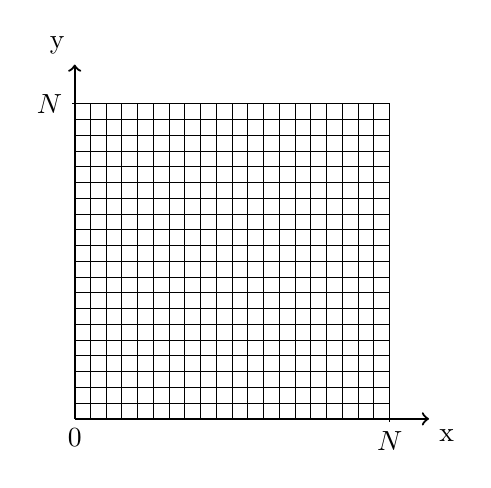
\begin{tikzpicture}
        \draw[step=0.2cm,black] (0,0) grid (4,4);
        \draw[thick,->] (0,0) -- (4.5,0) node[anchor=north west] {x};
        \draw[thick,->] (0,0) -- (0,4.5) node[anchor=south east] {y};
        \draw (4cm,1pt) -- (4cm,-1pt) node[anchor=north] {$N$};
        \draw (1pt,4cm) -- (-1pt,4cm) node[anchor=east] {$N$};
        \draw (0,0) -- (0,0) node[anchor=north] {$0$};
      \end{tikzpicture}
    \caption{An $N \times N$ image on the image plane}
    \end{subfigure}
    \begin{subfigure}{.05\textwidth}
      \centering
      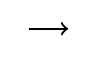
\begin{tikzpicture}
        \draw[thick,->] (0,0) -- (0.5,0);
      \end{tikzpicture}
    \end{subfigure}
    \begin{subfigure}{.50\textwidth}
      \centering
        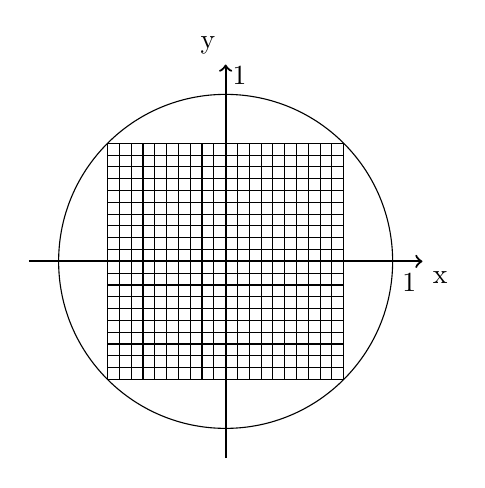
\begin{tikzpicture}
          \draw[step=0.15cm,black] (-1.5,-1.5) grid (1.5,1.5);
          \draw[thick,->] (-2.5,0) -- (2.5,0) node[anchor=north west] {x};
          \draw[thick,->] (0,-2.5) -- (0,2.5) node[anchor=south east] {y};
          \draw (0,0) circle (2.121cm);
          \draw (2.121cm,1pt) -- (2.121cm,-1pt) node[anchor=north west] {$1$};
          \draw (1pt,2.121cm) -- (-1pt,2.121cm) node[anchor=south west] {$1$};
        \end{tikzpicture}
      \caption{The image transformed inside the unit circle}
      \end{subfigure}
    \caption{The image before and after applying the transformation inside the unit disk}
    \label{fig:transform1}
\end{figure}

There are two "natural" ways to linearly transform a square image from image coordinates to polar coordinates inside the unit circle, using only translation and scaling~\cite{kintner}.

The first method is to transform the entire image inside the unit circle, as shown on Figure~\ref{fig:transform1}. This way all of the pixels will be used for calculating the (quaternion) moments, but some areas of the unit disk will remain empty, no pixels fall on those areas.

The other method is to transform the image such that the unit disk becomes the inscribed circle of the square image, as shown on Figure~\ref{fig:transform2}. This method fills the entire unit disk with pixels, but some pixels fall outside the unit circle and thus will not be used for the calculation of (quaternion) moments.

The polar coordinates $(r,\theta)$ corresponding to the image coordinates $(x,y)$ can be calculated by the following formulas, which is the mapping proposed by \citeauthor{Chong}~\cite{Chong}:
\begin{gather*}
  r = \sqrt{(c_1x + c_2)^2 + (c_1y + c_2)^2}, \\
  \theta = \tan^{-1}\left(\frac{c_1y + c_2}{c_1x + c_2}\right),
\end{gather*}
where $c_1$, $c_2 \in \mathds{R}$ depend on which of the previously mentioned transformations is used. A $\lambda \in \mathds{R}$ scaling factor is also defined for each transformation.
For the first one (Figure~\ref{fig:transform1}): $c_1 = \frac{\sqrt{2}}{N - 1}$, $c_2 = -\frac{1}{\sqrt{2}}$, and $\lambda = \frac{2}{\pi}$, while for the other transformation (Figure~\ref{fig:transform2}): $c_1 = \frac{2}{N - 1}$, $c_2 = -1$ and $\lambda = 1$, where $N$ is the number of pixels along each axis of the image.
  
\begin{figure}[tb]
    \begin{subfigure}{.43\textwidth}
    \centering
      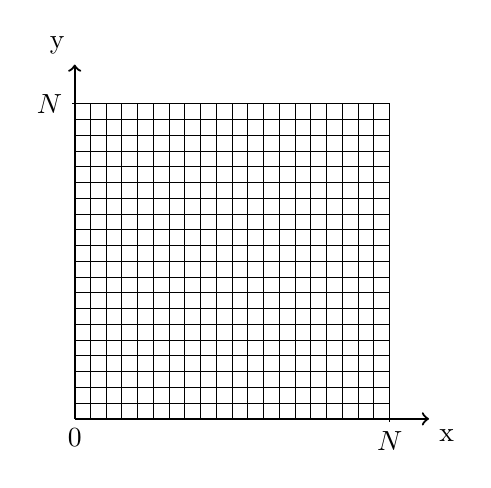
\begin{tikzpicture}
        \draw[step=0.2cm,black] (0,0) grid (4,4);
        \draw[thick,->] (0,0) -- (4.5,0) node[anchor=north west] {x};
        \draw[thick,->] (0,0) -- (0,4.5) node[anchor=south east] {y};
        \draw (4cm,1pt) -- (4cm,-1pt) node[anchor=north] {$N$};
        \draw (1pt,4cm) -- (-1pt,4cm) node[anchor=east] {$N$};
        \draw (0,0) -- (0,0) node[anchor=north] {$0$};
      \end{tikzpicture}
    \caption{An $N \times N$ image on the image plane}
    \end{subfigure}
    \begin{subfigure}{.05\textwidth}
      \centering
      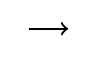
\begin{tikzpicture}
        \draw[thick,->] (0,0) -- (0.5,0);
      \end{tikzpicture}
    \end{subfigure}
    \begin{subfigure}{.50\textwidth}
      \centering
        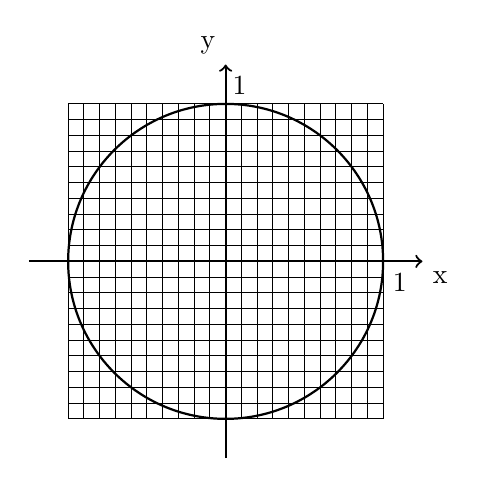
\begin{tikzpicture}
          \draw[thin,step=0.2cm,black] (-2,-2) grid (2,2);
          \draw[thick,->] (-2.5,0) -- (2.5,0) node[anchor=north west] {x};
          \draw[thick,->] (0,-2.5) -- (0,2.5) node[anchor=south east] {y};
          \draw[thick] (0,0) circle (2cm);
          \draw (2cm,1pt) -- (2cm,-1pt) node[anchor=north west] {$1$};
          \draw (1pt,2cm) -- (-1pt,2cm) node[anchor=south west] {$1$};
        \end{tikzpicture}
      \caption{The image transformed onto the unit disk}
      \end{subfigure}
    \caption{The image before and after applying the transformation onto the unit disk}
    \label{fig:transform2}
\end{figure}


The system of points defined by performing either one of these transformations for the entire image can be used as the basis points for the discretization, or the pixel values at these points can be used to approximate the values of the image function at other points on the unit disk using interpolation techniques. 


\subsection{Discretization of QZMs}
In general, using the polar form of the transformed coordinates, the continuous integral of \eqref{eq:QZRM} can be replaced by discrete approximations of form
\begin{equation}\label{eq:QZMappr}
	Z_{n,m}^R(f) \approx \lambda_{n,m} \sum_{k=1}^{N_1} \sum_{j=1}^{N_2} f(r_k,\theta_j) \phi_{n,m}(r_k,\theta_j) w(r_k,\theta_j),
\end{equation}
with some discretization weight function $w$ and normalization constants $\lambda_{n,m}$. In this discretization formula, the system of points $(r_k,\theta_j)$ does not necessarily coincide with the transformed lattice of the pixels, so $f(r_k,\theta_j)$ is some approximation of the image function, calculated from the discrete pixel values.


Using either one of the previously defined "natural" transformations, a point system on the unit disk can be obtained. The approximation of the image function $f$ at these points is not necessary as each point can have the corresponding pixel value assigned to it. Using this point system in \eqref{eq:QZMappr}, the following formula can be used to approximate the QZMs of the original image function:
\begin{gather*}
    Z_{n,m}^R(f) \approx \lambda\frac{n + 1}{(N - 1)^2}\sum_{x = 0}^{N-1}\sum_{y = 0}^{N-1}R_{n,m}(r_{x,y})f(x,y)e^{-\bm{\mu}m\theta_{x,y}},
\end{gather*}
where the RGB image $f \in \mathds{R}^2 \rightarrow \mathds{H}$ is now defined in image coordinates, $(r_{x,y},\theta_{x,y})$ are the polar coordinates belonging to the image coordinates $(x,y)$, and $\lambda$ is the previously defined scaling factor belonging to the linear image transformation.

In the rest of this thesis, for comparison purposes, the transformation of the image inside the unit circle (Figure~\ref{fig:transform1}) will be used as \citeauthor{qzmi}~\cite{qzmi} used this discretization to present their results.

\paragraph{Discrete orthogonality.}
Even though the (quaternion-valued) Zernike functions are a set of orthogonal functions on the complex unit disk, neither of the previously defined point systems provide discrete orthogonality, meaning that the discretization of the orthogonality relations in \eqref{Zortho} and \eqref{QZortho} over these point systems is not satisfied.


This lack of discrete orthogonality results in poor performance of the methods, especially under noisy conditions. It also makes the moment representation of an image redundant, hence introducing unwanted errors during image reconstruction.


A method for the discretization of the quaternion-valued Zernike functions, providing discrete orthogonality is proposed in Chapter~\ref{sec:maths}.

\subsection{Discretization of QRHFMs}
\citeauthor{LiuAcc}~\cite{LiuAcc} defined a point system for the discretization of quaternion radial harmonic Fourier moments, which consists of equally spaced radii and uniformly distributed points along these radii:
\begin{gather*}
    (r_u, \theta_v) = \left(\frac{u}{N}, \frac{2\pi v}{N}\right), \qquad u = 0,1,\ldots ,N - 1, \qquad v = 0,1,\ldots ,N - 1,
\end{gather*}
where $N$ is the number of pixels along each axis in the original image. The value of the image function $f$ can be approximated at these points by assigning the value of the closest pixel to each point:
\begin{gather*}
    f(r_u, \theta_v) \approx f'\left(\left \lfloor r_u\frac{N}{2}\sin \theta_v \right \rfloor + \frac{N}{2}, \left \lfloor r_u\frac{N}{2}\cos \theta_v \right \rfloor + \frac{N}{2}\right),
\end{gather*}
where $f'$ denotes the original image, given in image coordinates.


Using this system of points for the discretization of the integrals in \eqref{eq:QRHFM}, we get
\begin{gather*}
    F_{n,m}^R(f) \approx \frac{4}{2\pi N^2}\sum_{u = 0}^{N-1}\sum_{v = 0}^{N-1}f(r_u, \theta_v)H_{n,m}^*(r_u, \theta_v).
\end{gather*}


The basis functions $H_{n,m}$ satisfy the discrete orthogonality relation with this method of discretization, thus no additional error is introduced by the discretization.

\subsection{Other discretization methods}
The "natural" method of discretization (as described in the case of QZMs) proved to be susceptible to inaccuracies of both geometric and numeric nature when applied to grayscale images. \citeauthor{LiaoPawlak} described these issues in the case of the conventional Zernike moments~\cite{LiaoPawlak,PawlakLiao}. These problems are inherited by the quaternion generalizations as well. 


Later, \citeauthor{Xin}~\cite{Xin} proposed a more accurate computational technique, where the unit disk $\D$ is partitioned into polar sector of approximately equal areas. The original pixels are transformed to the centroids of these sectors via cubic interpolation. The weights for the discretization can be computed by integrating the $\phi_{n,m}$ basis functions over the respective polar sectors.


The same idea, adapted to quaternion-type moments for any aforementioned radial system could substantially improve the performance of tasks like image reconstruction, as well as recognition after RST transformations and addition of different kinds of noise. The reason for this is the improved accuracy gained for the computation of respective moments and invariants. Examples of this technique applied for color images include the papers of \citeauthor{HosnyLegendre} for Legendre \cite{HosnyLegendre} and Chebyshev \cite{HosnyChebyshev} radial systems.


A significant drawback of this approach is that the cubic interpolation used for coordinate transformation is irreversible. This means that in order to reconstruct the original image some other transformation has to be used. This additional transformation can further introduce error during image reconstruction. 
To circumvent this issue, in previous works \cite{LiaoPawlak,PawlakLiao,Xin,HosnyLegendre,HosnyChebyshev}, the error of reconstruction was measured for the transformed image and its reconstructions on the unit disk $\D$ only. 


Another, although minor issue is the natural smoothing provided by the cubic interpolation, which unintentionally improves the obtained results for experiments on noisy images by filtering some of the noise. This is a sometimes unwanted side effect, which can distort measurements of the performance of the moments themselves. To ensure fair comparisons with the previously introduced "natural" transformations, linear interpolation should be used, ensuring invertible coordinate transformations, and also excluding unwanted side effects.


Finally, the results of \citeauthor{WangAcc} \cite{WangAcc} and \citeauthor{LiuAcc} \cite{LiuAcc} for radial harmonic Fourier moments (as described previously) are some of the recent advances in the study of quaternion moments, introducing a novel coordinate transformation, which improves accuracy for this specific function system while maintaining fast computation times, without utilizing cubic interpolation at all. These improvements stem from the discrete orthogonality provided by the novel coordinate transformation, with respect to the specific basis functions.

\section{Applications}
In this section, we list some practical applications of image moments and moment invariants, with special attention to Zernike moments.
Zernike moments and moment invariants are a useful tool in optical and medical applications. Specifically, Zernike moments can be used to represent and capture optical aberrations~\cite{wavefront,optical_human_eye,opt_surf}.

Furthermore, applications in pattern recognition have shown that in noisy environments Zernike moment yield the best results~\cite{pattern_recognition}. \citeauthor{hand_vein}~\cite{hand_vein} have used Zernike moment invariants to extract descriptions of hand vein patterns.

Another field of application is image watermarking, where a watermark that is resistant against transformation- and noise-based attacks may be inserted directly into the moment decomposition of an image~\cite{watermarking_auth, robust_watermarking, invariant_watermark}.

Finally, one potentially powerful application is to use Zernike moments in conjunction with neural networks. The robustness of neural networks with respect to noise is a known shortcoming of current systems~\cite{nn_robust,nn_noise_robust}. Zernike moments can be used as some components of the feature vector input of neural networks, thus providing their high robustness to noise during forward propagation~\cite{zernike_nn,zernike_nn2}. 
